% Build from the repository root:
%   pdflatex -interaction=nonstopmode -halt-on-error -output-directory=/tmp/epilink-texbuild docs/epilink_schematic.tex
%   magick -density 300 /tmp/epilink-texbuild/epilink_schematic.pdf -background white -alpha remove -alpha off docs/epilink_schematic.png
%
% This schematic redraws the scenario families from docs/epilink_scenarios.svg
% directly in TikZ so the workflow figure remains a single TeX source.
\documentclass[tikz,border=10pt]{standalone}

\usepackage[T1]{fontenc}
\usepackage{amsmath}
\usepackage{microtype}
\usepackage{newtxtext,newtxmath}
\usepackage{xcolor}
\usetikzlibrary{arrows.meta,calc,positioning,shapes.multipart}

\definecolor{Ink}{HTML}{21374A}
\definecolor{Subtle}{HTML}{61788E}
\definecolor{ContainerStroke}{HTML}{B9C6D5}
\definecolor{NeutralStroke}{HTML}{4C6880}
\definecolor{NeutralBand}{HTML}{E7EEF4}
\definecolor{BlueStroke}{HTML}{2D72A8}
\definecolor{BlueFill}{HTML}{EEF7FF}
\definecolor{BlueBand}{HTML}{D8EAFF}
\definecolor{VioletStroke}{HTML}{6C51B3}
\definecolor{VioletFill}{HTML}{F5F0FF}
\definecolor{VioletBand}{HTML}{E7DBFF}
\definecolor{GreenStroke}{HTML}{2F855A}
\definecolor{GreenFill}{HTML}{EFF9F1}
\definecolor{GreenBand}{HTML}{DDF2E2}
\definecolor{AmberStroke}{HTML}{C76C2C}
\definecolor{AmberFill}{HTML}{FFF5E8}
\definecolor{AmberBand}{HTML}{FFE3C6}

\tikzset{
  flow/.style={
    -{Latex[length=3.6mm,width=2.8mm]},
    draw=Ink,
    line width=1.05pt,
    shorten >= 2pt,
    shorten <= 2pt
  },
  scenario flow/.style={
    -{Latex[length=2.6mm,width=2.0mm]},
    draw=Ink,
    line width=0.85pt,
    shorten >= 1.2pt,
    shorten <= 1.2pt
  },
  workflow box/.style={
    rounded corners=10pt,
    very thick,
    rectangle split,
    rectangle split parts=2,
    rectangle split part align={left,left},
    font=\small,
    inner sep=7pt,
    align=left,
    outer sep=0pt,
    text=Ink
  },
  neutral box/.style={
    workflow box,
    draw=NeutralStroke,
    rectangle split part fill={NeutralBand,white}
  },
  blue box/.style={
    workflow box,
    draw=BlueStroke,
    rectangle split part fill={BlueBand,BlueFill}
  },
  violet box/.style={
    workflow box,
    draw=VioletStroke,
    rectangle split part fill={VioletBand,VioletFill}
  },
  green box/.style={
    workflow box,
    draw=GreenStroke,
    rectangle split part fill={GreenBand,GreenFill}
  },
  amber box/.style={
    workflow box,
    draw=AmberStroke,
    rectangle split part fill={AmberBand,AmberFill}
  },
  sampled case/.style={
    circle,
    draw=Ink,
    fill=white,
    line width=0.9pt,
    minimum size=6.7mm,
    inner sep=0pt,
    font=\scriptsize,
    text=Ink
  },
  latent case/.style={
    sampled case,
    fill=black!10
  }
}

\begin{document}
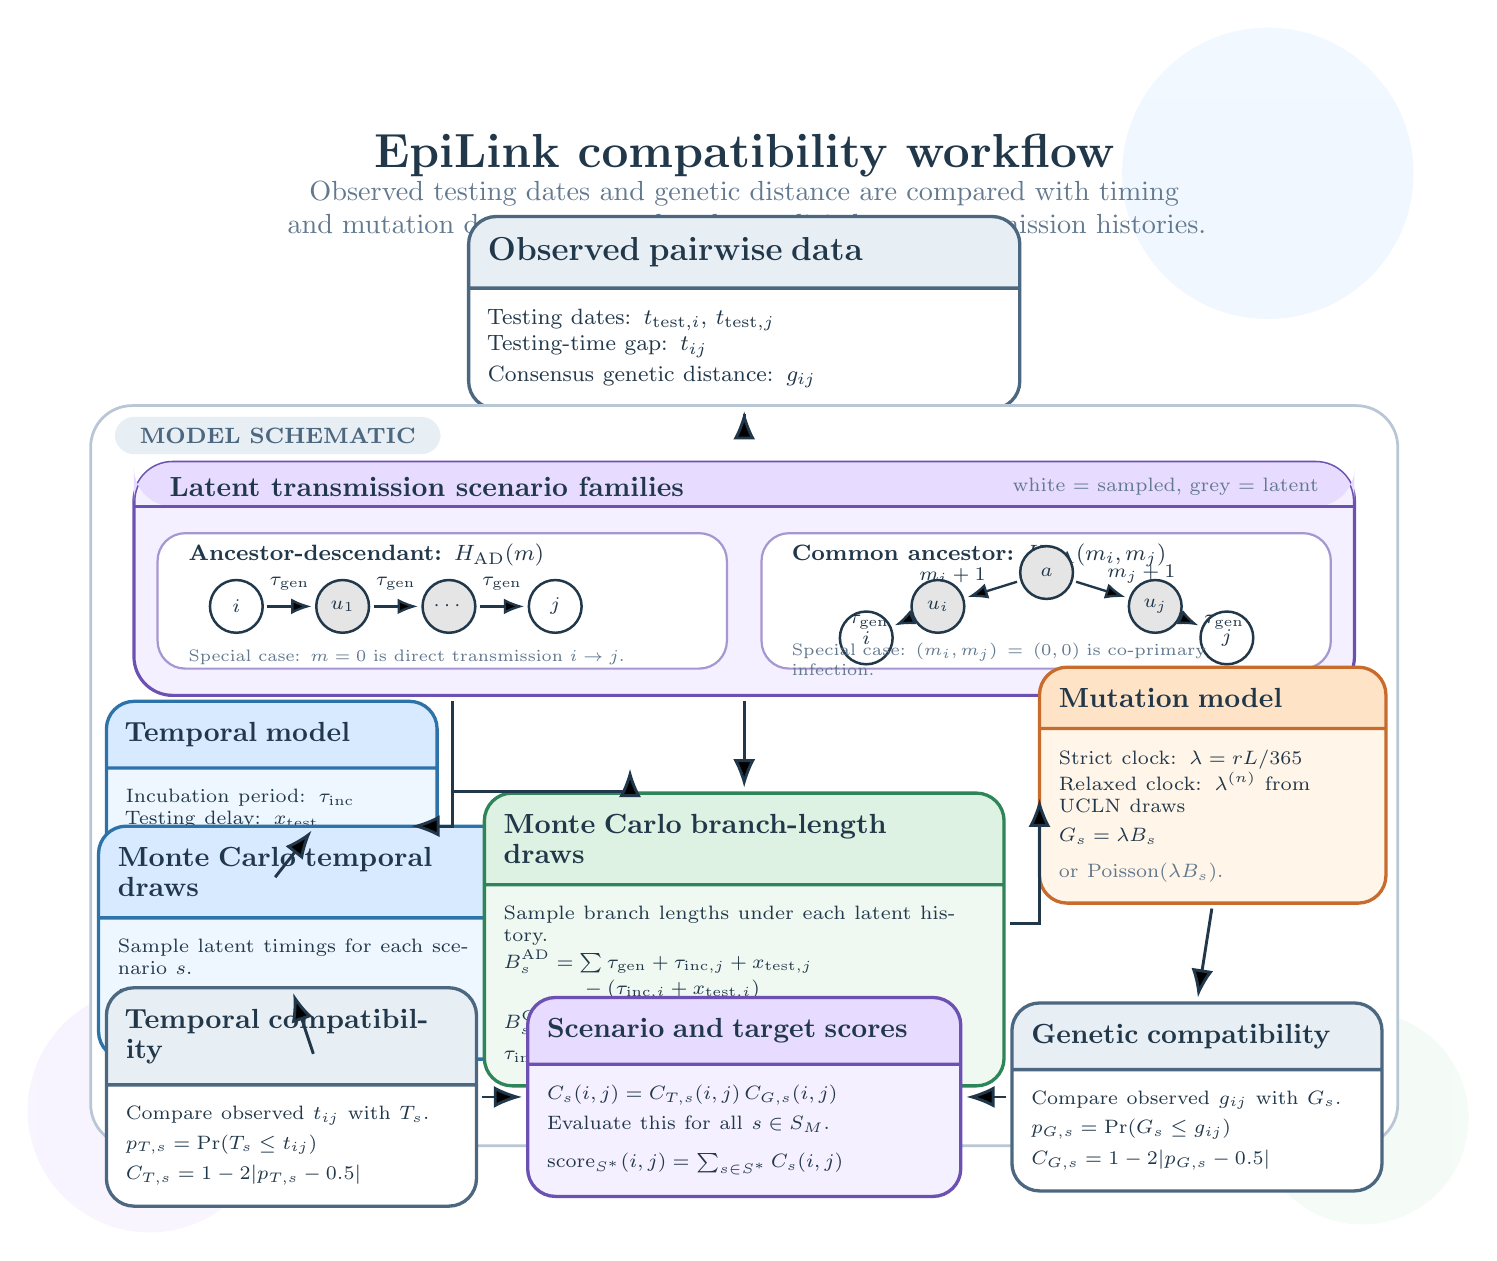
\begin{tikzpicture}[x=1cm,y=1cm]
  \fill[white] (0,0) rectangle (18,14);
  \fill[BlueBand, opacity=0.35] (15.65, 13.05) circle (1.85cm);
  \fill[VioletBand, opacity=0.28] (1.45, 1.15) circle (1.55cm);
  \fill[GreenBand, opacity=0.30] (16.85, 1.05) circle (1.35cm);

  \node[align=center, text=Ink] at (9.0, 13.28) {\LARGE\bfseries EpiLink compatibility workflow};
  \node[
    align=center,
    text=Subtle,
    text width=15.8cm
  ] at (9.0, 12.58) {\normalsize
    Observed testing dates and genetic distance are compared with timing and mutation draws
    generated under explicit latent transmission histories.
  };

  \node[
    neutral box,
    text width=6.2cm,
    minimum width=7.0cm
  ] (input) at (9.0, 11.28) {%
    {\large\bfseries Observed pairwise data}
    \nodepart{second}
    {\footnotesize
      Testing dates: $t_{\mathrm{test},i}$, $t_{\mathrm{test},j}$\\
      Testing-time gap: $t_{ij}$\\
      Consensus genetic distance: $g_{ij}$
    }
  };

  \draw[
    rounded corners=15pt,
    line width=1.0pt,
    draw=ContainerStroke,
    fill=white
  ] (0.70, 0.70) rectangle (17.30, 10.10);

  \node[
    anchor=west,
    rounded corners=7pt,
    fill=NeutralBand,
    inner xsep=9pt,
    inner ysep=4pt,
    text=NeutralStroke,
    font=\bfseries\footnotesize
  ] at (1.00, 9.72) {MODEL SCHEMATIC};

  \coordinate (modeltop) at (9.0, 10.10);
  \draw[flow] (input.south) -- (modeltop);

  % Scenario panel sourced from the latent-history figure.
  \path[
    draw=VioletStroke,
    fill=VioletFill,
    rounded corners=14pt,
    line width=1.15pt
  ] (1.25, 6.42) rectangle (16.75, 9.38);
  \path[
    fill=VioletBand,
    rounded corners=14pt
  ] (1.25, 8.82) rectangle (16.75, 9.38);
  \draw[VioletStroke, line width=0.8pt] (1.25, 8.82) -- (16.75, 8.82);
  \node[anchor=west, font=\bfseries\normalsize, text=Ink] at (1.58, 9.07) {Latent transmission scenario families};
  \node[anchor=east, font=\scriptsize, text=Subtle] at (16.42, 9.07) {white = sampled, grey = latent};

  \path[
    draw=VioletStroke!60,
    fill=white,
    rounded corners=10pt,
    line width=0.8pt
  ] (1.55, 6.76) rectangle (8.78, 8.48);
  \path[
    draw=VioletStroke!60,
    fill=white,
    rounded corners=10pt,
    line width=0.8pt
  ] (9.22, 6.76) rectangle (16.45, 8.48);

  \node[anchor=west, font=\bfseries\footnotesize, text=Ink] at (1.82, 8.20) {Ancestor-descendant: $H_{\mathrm{AD}}(m)$};

  \node[sampled case] (adi) at (2.55, 7.55) {$i$};
  \node[latent case] (adu) at (3.90, 7.55) {$u_1$};
  \node[latent case] (addots) at (5.25, 7.55) {$\cdots$};
  \node[sampled case] (adj) at (6.60, 7.55) {$j$};
  \draw[scenario flow] (adi) -- (adu) node[midway, above=2pt, font=\scriptsize, text=Ink] {$\tau_{\mathrm{gen}}$};
  \draw[scenario flow] (adu) -- (addots) node[midway, above=2pt, font=\scriptsize, text=Ink] {$\tau_{\mathrm{gen}}$};
  \draw[scenario flow] (addots) -- (adj) node[midway, above=2pt, font=\scriptsize, text=Ink] {$\tau_{\mathrm{gen}}$};
  \node[
    anchor=west,
    font=\fontsize{6.5}{7.5}\selectfont,
    text=Subtle,
    text width=6.1cm,
    align=left
  ] at (1.82, 6.90) {Special case: $m=0$ is direct transmission $i \rightarrow j$.};

  \node[anchor=west, font=\bfseries\footnotesize, text=Ink] at (9.48, 8.20) {Common ancestor: $H_{\mathrm{CA}}(m_i, m_j)$};

  \node[latent case] (caa) at (12.84, 7.98) {$a$};
  \node[latent case] (caui) at (11.46, 7.55) {$u_i$};
  \node[latent case] (cauj) at (14.22, 7.55) {$u_j$};
  \node[sampled case] (cai) at (10.55, 7.15) {$i$};
  \node[sampled case] (caj) at (15.13, 7.15) {$j$};
  \draw[scenario flow] (caa) -- (caui) node[midway, above left=-2pt, font=\scriptsize, text=Ink] {$m_i + 1$};
  \draw[scenario flow] (caa) -- (cauj) node[midway, above right=-2pt, font=\scriptsize, text=Ink] {$m_j + 1$};
  \draw[scenario flow] (caui) -- (cai) node[midway, left=1pt, font=\scriptsize, text=Ink] {$\tau_{\mathrm{gen}}$};
  \draw[scenario flow] (cauj) -- (caj) node[midway, right=1pt, font=\scriptsize, text=Ink] {$\tau_{\mathrm{gen}}$};
  \node[
    anchor=west,
    font=\fontsize{6.5}{7.5}\selectfont,
    text=Subtle,
    text width=5.6cm,
    align=left
  ] at (9.48, 6.88) {Special case: $(m_i, m_j)=(0,0)$ is co-primary infection.};

  \coordinate (scenario south left) at (5.30, 6.42);
  \coordinate (scenario south center) at (9.0, 6.42);

  \node[
    blue box,
    text width=3.5cm,
    minimum width=4.2cm
  ] (temporal) at (3.00, 5.20) {%
    {\normalsize\bfseries Temporal model}
    \nodepart{second}
    {\scriptsize
      Incubation period: $\tau_{\mathrm{inc}}$\\
      Testing delay: $x_{\mathrm{test}}$\\
      Generation time: $\tau_{\mathrm{gen}}$
    }
  };

  \node[
    amber box,
    text width=3.7cm,
    minimum width=4.4cm
  ] (mutation) at (14.95, 5.28) {%
    {\normalsize\bfseries Mutation model}
    \nodepart{second}
    {\scriptsize
      Strict clock: $\lambda = rL/365$\\
      Relaxed clock: $\lambda^{(n)}$ from UCLN draws\\[0.30em]
      $G_s = \lambda B_s$\\[0.25em]
      \textcolor{Subtle}{or $\operatorname{Poisson}(\lambda B_s)$.}
    }
  };

  \node[
    blue box,
    text width=4.8cm,
    minimum width=5.5cm
  ] (tempdraws) at (3.55, 3.28) {%
    {\normalsize\bfseries Monte Carlo temporal draws}
    \nodepart{second}
    {\scriptsize
      Sample latent timings for each scenario $s$.\\[0.25em]
      $T_s = A_j(s)-A_i(s)+\tau_{\mathrm{inc},j}+x_{\mathrm{test},j}$\\
      $\phantom{T_s = {}}-\tau_{\mathrm{inc},i}-x_{\mathrm{test},i}$
    }
  };

  \node[
    green box,
    text width=5.9cm,
    minimum width=6.6cm
  ] (branchdraws) at (9.0, 3.32) {%
    {\normalsize\bfseries Monte Carlo branch-length draws}
    \nodepart{second}
    {\scriptsize
      Sample branch lengths under each latent history.\\[0.20em]
      $B_s^{\mathrm{AD}} = \sum \tau_{\mathrm{gen}} + \tau_{\mathrm{inc},j} + x_{\mathrm{test},j}$\\
      $\phantom{B_s^{\mathrm{AD}} = {}}-(\tau_{\mathrm{inc},i}+x_{\mathrm{test},i})$\\[0.20em]
      $B_s^{\mathrm{CA}} = \sum \tau_{\mathrm{gen}}^{(i)} + \sum \tau_{\mathrm{gen}}^{(j)} + \tau_{\mathrm{inc},i} + x_{\mathrm{test},i} + \tau_{\mathrm{inc},j} + x_{\mathrm{test},j}$
    }
  };

  \node[
    neutral box,
    text width=4.0cm,
    minimum width=4.7cm
  ] (temporalcompat) at (3.25, 1.32) {%
    {\normalsize\bfseries Temporal compatibility}
    \nodepart{second}
    {\scriptsize
      Compare observed $t_{ij}$ with $T_s$.\\[0.35em]
      $p_{T,s} = \operatorname{Pr}(T_s \le t_{ij})$\\
      $C_{T,s} = 1 - 2\lvert p_{T,s} - 0.5 \rvert$
    }
  };

  \node[
    violet box,
    text width=4.8cm,
    minimum width=5.5cm
  ] (scores) at (9.0, 1.32) {%
    {\normalsize\bfseries Scenario and target scores}
    \nodepart{second}
    {\scriptsize
      $C_s(i,j) = C_{T,s}(i,j)\,C_{G,s}(i,j)$\\[0.35em]
      Evaluate this for all $s \in S_M$.\\[0.35em]
      $\operatorname{score}_{S^\ast}(i,j) = \sum_{s \in S^\ast} C_s(i,j)$
    }
  };

  \node[
    neutral box,
    text width=4.0cm,
    minimum width=4.7cm
  ] (geneticcompat) at (14.75, 1.32) {%
    {\normalsize\bfseries Genetic compatibility}
    \nodepart{second}
    {\scriptsize
      Compare observed $g_{ij}$ with $G_s$.\\[0.35em]
      $p_{G,s} = \operatorname{Pr}(G_s \le g_{ij})$\\
      $C_{G,s} = 1 - 2\lvert p_{G,s} - 0.5 \rvert$
    }
  };

  \draw[flow] (temporal.south) -- (tempdraws.north);
  \draw[flow] (scenario south left) |- ([xshift=1.15cm]tempdraws.north);
  \draw[flow] (scenario south center) -- (branchdraws.north);
  \draw[flow] ([xshift=0.15cm]temporal.east) -| ([xshift=-1.45cm,yshift=0.38cm]branchdraws.north);
  \draw[flow] ([yshift=0.20cm]branchdraws.east) -| ([yshift=-0.10cm]mutation.west);
  \draw[flow] (tempdraws.south) -- (temporalcompat.north);
  \draw[flow] (mutation.south) -- (geneticcompat.north);
  \draw[flow] (temporalcompat.east) -- (scores.west);
  \draw[flow] (geneticcompat.west) -- (scores.east);
\end{tikzpicture}
\end{document}
